\chapter{Analysis, Results and Discussion}
\section{Calibration of the X-ray energy detector (RED)}
\subsection{Calibration using a tungsten X-ray tube}
The goniometer is set to an angle of 0\degree to record a calibration spectrum. In the spectrum two clear peaks, corresponding to the characteristic tungsten $L_\alpha$ and $L_\beta$, are visible. The energy of these lines is known from literature and saved in the MEASURE software. Using this software, we can place markers to the corresponding peaks to determine a calibration equation, which energy to channel numbers. The calibration equation turned out to be: $$E = \SI{0.03}{\frac{keV}{channel}} \cdot a + \SI{0.03}{keV}$$
where a is the channel number. 
We were advised to place the markers in such a way that the offset in the calibration equation is close to zero.
\subsection{Evaluation of the calibration using standard samples}
To evaluate the calibration determined in the first part, the goniometer is set to an angle of 45\degree and the spectra of multiple standard samples is recorded. The energy of the measured peaks can then be compared to literature values. As it is hardly possible to do a proper double gaussian fit on overlapping peaks using the MEASURE software, the data was fitted using Python and kafe2 to determine the energy of each peak. The results are displayed in table \ref{table:maxcalib} and the fits displayed in the appendix chapter \ref{appendix:calib}
\begin{table}[H]
    \centering
    \label{table:maxcalib}
    \caption{fit results and literature values}
    \begin{tabular}{ccccccc}
    
        sample & peak &a in keV&b&c& closest literature value in keV &closest line\\\hline
        Fe &1 & 12.45& 1.21&64.54 & 7.05&$K_{\beta_1}$  \\
           & 2& 12.79& 0.36&47.06 & 7.05 &$K_{\beta_1}$ \\
        Ni & 1&14.85 &0.43 &75.24 & 8.26 &$K_{\beta_1}$ \\
           & 2& 14.52& 1.32 &85.39 & 8.26 & $K_{\beta_1}$ \\
        Cu & 1&15.98 & 0.35& 65.55&  8.90 & $K_{\beta_1}$\\
           & 2& 15.68&1.31 & 90.45 &  8.90 &$K_{\beta_1}$\\
        Zn & 1& 17.12&  0.36& 65.68 &  9.57 &$K_{\beta_1}$ \\
           & 2&16.88 & 1.37& 99.26&  9.57 & $K_{\beta_1}$\\
        Pb & 1&24.70 &0.92 &25.13 &  14.76 &$K_{\gamma_1}$ \\
           & 2&20.55&1.20 &28.95 &  14.76 &$K_{\gamma_1}$ \\\hline
        \end{tabular}
    
\end{table}
\begin{figure}[]

    \centering
    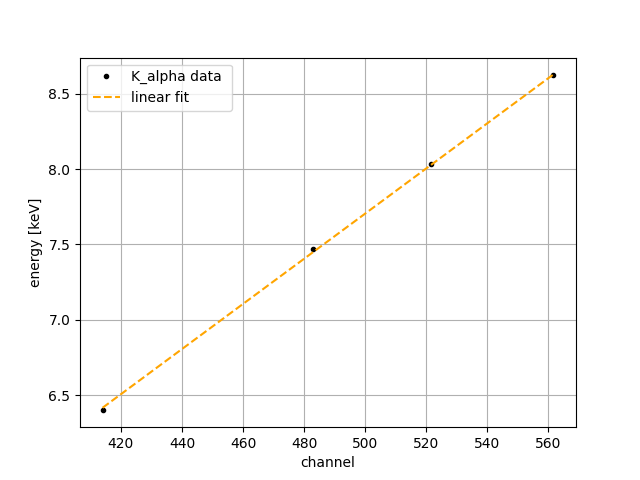
\includegraphics[width=110mm,scale=0.5]{MAX/include/K_alpha.png}
    \caption{A second calibration fit}
    \label{figure:Kalpha fit}
\end{figure}
\begin{figure}[]


    \centering
    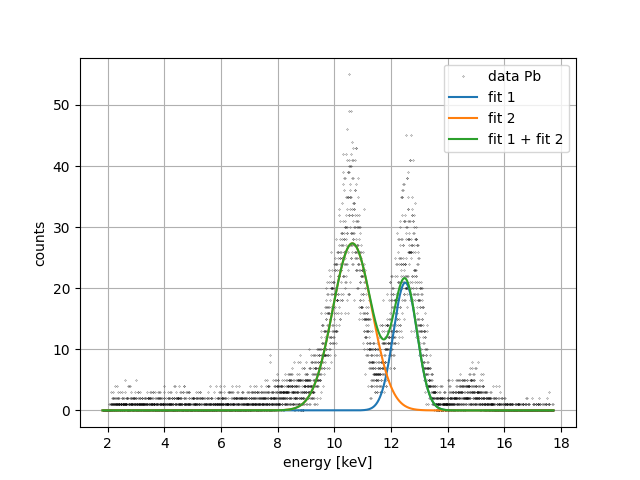
\includegraphics[width=110mm,scale=0.5]{MAX/include/plotsPb2.png}
    \caption{The new calibration applied to the lead spectrum}
    \label{figure:lead comp}
\end{figure}
As seen in the table, the calibration fails to deliver the correct energy of the characteristic lines for every sample material. It is very likely that the markers for calibration in the first task were set incorrectly.

In order to gain a usable calibration, the channel numbers of peaks were matched with the theoretical expected energy values of the $K_{\alpha}$ lines. The data was then fitted to a linear curve which yields the calibration equation: $$ E = \SI{0.015}{\frac{keV}{channel}} \cdot a + \SI{0.2214}{keV}$$
A plot of the fit can be seen in figure \ref{figure:Kalpha fit}. The literature values were taken from \cite{Xraylines}


This calibration is used in all tasks going further. \\Using the measured and theoretical lead data as a test for the calibration, one can see from figure \ref{figure:lead comp} that the calibration cannot produce the correct energies for the peaks. The calibration can therefore only be used for elements of roughly the same atomic mass of iron. 


\section{Determination of the energy resolution of the RED}
To determine the energy resolution of the RED, multiple spectra of zinc at varying emission currents $I_e$ are measured. From the center of gravity and FWHM of the $K_\alpha$ line the resolution is determined using 
$$r = \frac{E_0}{\Delta E_{FWHM}}$$. In accordance to the exercise description, the measurement duration and number of pulses is also noted. 
The center of gravity is determined from the fit parameter a, while the FWHM is determined by $\Delta E_{FWHM} = 2\sqrt{2\ln{2}}b$.
The results are shown in table \ref{tab:maxZNFIT}
\begin{table}[H]
    \centering
    \caption{fit results and resolution calculation}
    \begin{tabular}{ccccccccc}
    I in mA & T in s & number of pulses& a & b & c &E0 in keV & $\Delta E_{FWHM}$ in keV & r \\\hline
          001  & 141       &       20002       &  8.604 &   0.496  &  116.28 & 8.604  &  1.168      &     7.364  \\
          005  &  23      &        20006       &  8.547  &  0.493 &  112.08 &  8.547  &  1.162 & 7.352\\
          010  &  13    &         20016         & 8.629  &  0.523 &  106.54 &  8.629  &  1.232 & 7.003\\
          020  &   9    &           20056       & 8.388  &  0.544  & 99.74  &  8.388  &    1.282  & 6.541\\
          050  &   7    &            21824      & 8.037  &  0.632 &  92.04 &  8.037  &   1.488   & 5.398\\
          100  &   7    &             21824    &  10.931 &  0.698  & 75.87  &  10.931  &   1.644   & 6.649\\\hline
        
    \end{tabular}

    \label{tab:maxZNFIT}
\end{table}
\begin{figure}[H]
    
    \centering
    
    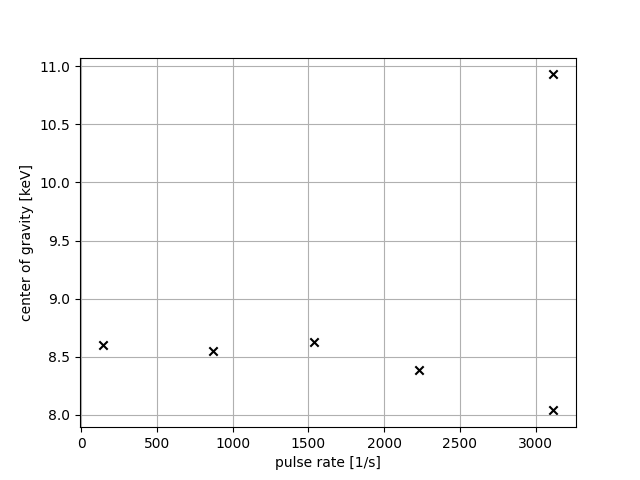
\includegraphics[width=110mm,scale=0.5]{MAX/include/cog.png}
    \caption{center of gravity over pulse rate}
    \label{figure:maxcog}
\end{figure}

\begin{figure}[H]
   
    \centering
     
    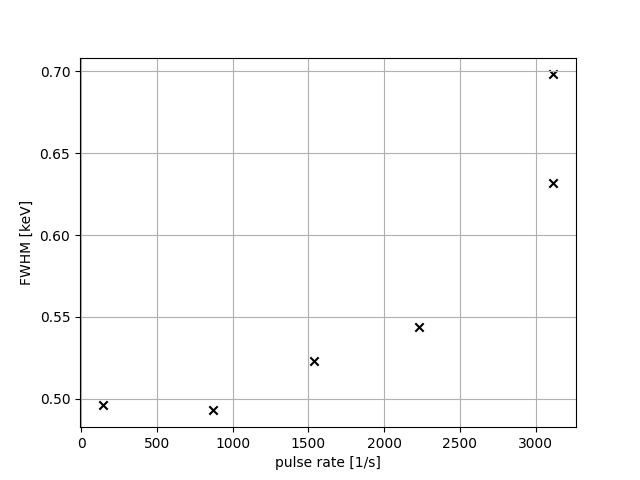
\includegraphics[width=110mm,scale=0.5]{MAX/include/fwhm.png}
    \caption{FWHM over pulse rate}
    \label{figure:maxFWHM}
\end{figure}
The center of gravity of the distribution and the FWHM are plotted against the pulse rate in figures \ref{figure:maxcog} and \ref{figure:maxFWHM}.


One can see that the FWHM rises greatly with the pulse rate, most likely because of the increased scattering rate. The pulse rate should therefore be kept underneath \SI{1500}{\frac{1}{s}}.
\section{Quantitative X-ray fluorescence analysis, Moseley constant}
As seen in chapter \ref{chapter:moseley}, there is a linear relation between $\sqrt{E}$ and $Z$. By plotting  $\sqrt{E}$ over $Z$, one can determine the Rydberg-constant $R_\infty$ from the slope and the screening constant from the offset with the following formulas:
$$R_\infty = \frac{4\cdot m^2}{3c\cdot h}$$
$$\sigma_{1,2} = \frac{2b}{\sqrt{3R_\infty\cdot c \cdot h}}$$ The uncertainty can be determined using gaussian error propagation. An uncertainty of \SI{10}{\%} is assumed on the energy.
The fit is shown in figure \ref{fig:ZFIT}, the fit and calculation results in table \ref{tab:ZGIT}
\begin{figure}[H]
    \centering
    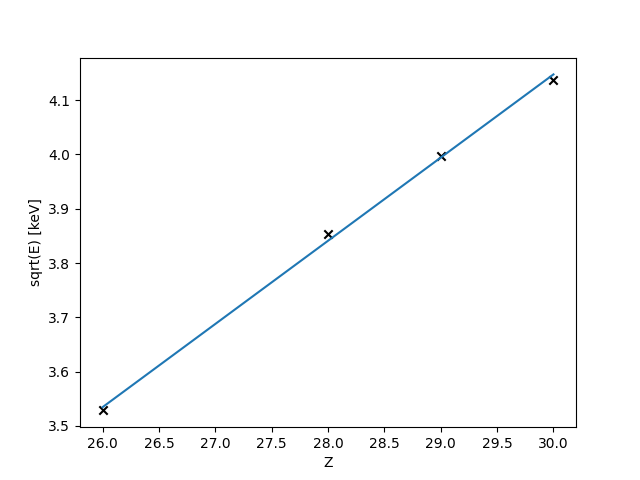
\includegraphics[width=110mm,scale=0.5]{MAX/include/lin.png}
    \caption{linear fit of $\sqrt{E}$ over Z}
    \label{fig:ZFIT}
\end{figure}
\begin{table}[H]
    \centering
    \caption{fit and calculation results}
    \begin{tabular}{cccc}
        m & b & $R_\infty$ in $\SI{}{\frac{1}{m}}$ & $\sigma_{1,2}$\\\hline
        $3.427 \pm 2.848$ & $-10.083 \pm 80.075$ & $(7.88 \pm 13.1)\cdot 10^{25}$ & $-2.94 \pm23.86$ \\\hline
    \end{tabular}
    
    \label{tab:ZGIT}
\end{table}
Comparing this with the literature value of \SI{10873731.568160(21)}{\frac{1}{m}}, one can see that the calculated result is magnitudes off. The screening constant seems to be negative, which is not what is physically expected, as the screening constant should shield off the charge of the nucleus. This is most likely caused by the faulty energy calibration done in the first task.



\section{Determination of the layer thickness of thin foils}
In accordance with the tutor, the reduced intensity mentioned in chapter \ref{section: determination} was not measured. The thickness of the foils covering the iron sample can therefore only be determined using the absorption law directly. In figure \ref{figure:foils} the measured peak intensities at different foil amounts are shown, as well as an exponential fit which yields the exponent.
$$ b = \mu\cdot \rho \cdot d \sqrt{2} = \SI{0.58 \pm 0.02}{\frac{1}{foils}}$$
using $\rho_{Al}= \SI{2.7}{\frac{g}{cm^3}}$ and $\mu_{Al} = \SI{92.8}{\frac{cm^2}{g}}$ one can now calculate the thickness. 
$$d = \frac{b}{\rho_{Al} \cdot \mu_{Al} \cdot \sqrt{2}} = \SI{16.36 \pm 0.56}{\mu m}$$
Commercially available aluminum foil usually has a thickness of $\SIrange[]{10}{15}{\mu m}$. The calculated result is most likely too high because the absorption of the radiation before it hits the iron sample was not taken into account. This absorption could have been taken into account by measuring the reduced intensity of X-rays travelling through just the foils. 

\begin{figure}[H]
   
    \centering
    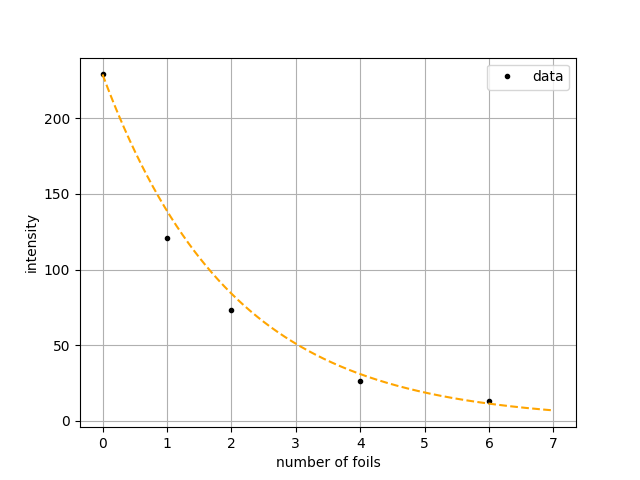
\includegraphics[width=110mm,scale=0.5]{MAX/include/foils.png}
    \caption{Intensity over foil amount}
    \label{figure:foils}
\end{figure}


\section{Qualitative X-ray fluorescence analysis on alloys}
The composition of the alloy solder and of a 5ct coin is to be determined. This is done by identifying the characteristic X-ray lines of elements in the spectra of each alloy. The concentration of each identified element can then be determined by dividing the element peak intensities by the sum of peak intensities of all identified elements. The measured spectra can be seen in figure \ref{figure:coin} and \ref{figure:lzinn}. \\

For the coin one can determine the peak of two elements, copper and nickel, with a respective concentration of $\SI{78.98}{\%}$ and $\SI{21.02}{\%}$. A 5ct coin is usually made of a steel core with a layer of copper. The concentration of copper seems plausible, however the concentration of nickel seems to be too high. The main component of steel, iron could not be identified in the spectrum. \\

For solder one can determine the peak of three elements, arsenic, krypton and yttrium with a respective concentration of \SI{48.19}{\%}, \SI{44.17}{\%} and \SI{7.64}{\%}. Solder usually consists of mainly zinc, sometimes lead, silver, copper or gold are added. The spectrum is incompatible with these elements. It is most likely that the sample was not positioned properly, as the amount of measured signals is very low. \\



\begin{figure}[H]
   
    \centering
    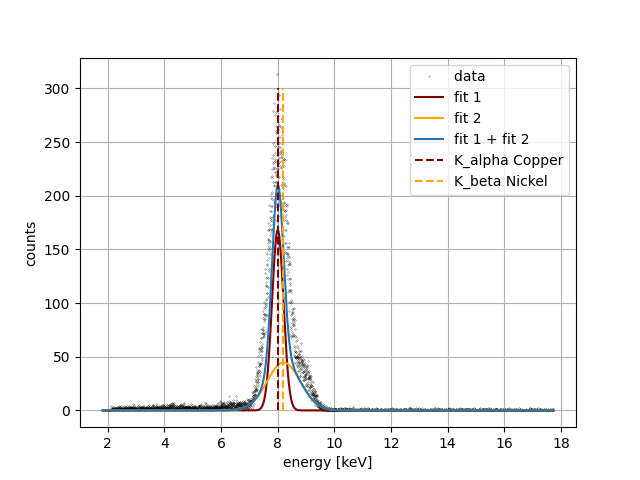
\includegraphics[width=110mm,scale=0.5]{MAX/include/plotsMuenze.png}
    \caption{Spectrum of a 5ct coin}
    \label{figure:coin}
\end{figure}

\begin{figure}[H]
   
    \centering
    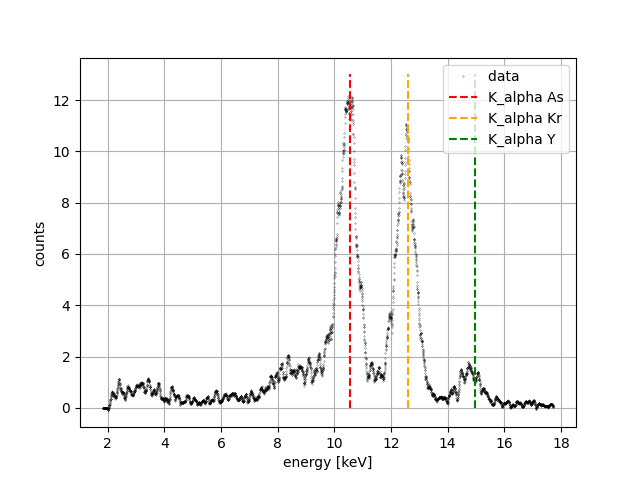
\includegraphics[width=110mm,scale=0.5]{MAX/include/plotslzinn.png}
    \caption{Spectrum of solder}
    \label{figure:lzinn}
\end{figure}